\section{Introduction}
 
Traditionally, the modelling of radiation damage has been confined to 
cases in which the radiation (i.e. a projectile) collides elastically with the 
nuclei of the target material. Collisions of this type are said to be 
dominated by nuclear stopping (energy transfer from the projectile 
to the nuclei). However, there are a broad range of scenarios (high 
energy collision cascades, swift heavy ion irradiation, and laser 
excitation) in which a significant portion (high energy collision cascades) 
or all (lasers and swift heavy ions) of the energy is transferred to the 
electrons in the target material. These cases, in which electronic stopping 
cannot be neglected, are impossible to account for using traditional 
molecular dynamics simulations (which assume equilibrium conditions 
between the target nuclei and electrons). This chapter describes the 
implementation of a hybrid continuum-atomistic implementation within \D 
that incorporates these electronic excitations.

The model is based on the traditional two-temperature model 
(TTM)~\cite{lifshits-60a}. This model splits the nuclei and electrons 
into two separate but interacting subsystems, each evolving according 
to a modified version of Fourier's heat equation. This continuum 
implementation is unable to track individual atomistic trajectories, thus 
information on superheating, recrystallisation, and pressure waves is lost. 
These limitations were overcome by Duffy and 
Rutherford~\cite{duffy-07a, duffy-09a}, by replacing 
the continuum representation of the lattice with an MD cell (the details of 
which will be described in this report). This model, known as the 
two-temperature molecular dynamics (2T-MD) model, has been successfully 
used to model high energy cascades in iron~\cite{zarkadoula-14a}, ultrafast 
laser irradiation of gold nanofilms~\cite{daraszewicz-13a}, and swift heavy ion 
irradiation of silicon~\cite{khara-16a}. 

\section{Methodology}

\subsection*{Electronic subsystem}

The electronic temperature is treated as a continuum system, and evolves 
according to Fourier's law of heat conduction:
\begin{equation} \label{eq:electronic_system}
C_e(T_e) \frac{\partial T_e}{\partial t} - \nabla . [\kappa_e \nabla T_e ] = -G_{ep}(T_e - T_i) + G_s T^{\prime}_i + A(r,t),
\end{equation}
where $C_e(T_e)$ is the electronic volumetric heat capacity (equal to the 
product of specific heat capacity and density), $\kappa_e$ is the 
electronic thermal conductivity, $G_{ep}(T_e)$ the electron-phonon 
coupling, $G_s$ the electronic stopping term (which is significant for 
lattice temperatures $T^{\prime}_i$ greater than a velocity cutoff, as defined later), 
and $A(r,t)$ the temporal and spatial dependent source term. This equation 
describes how energy evolves in the electronic system as follows: energy 
is dumped into the electronic system via the source term (for swift heavy 
ions and laser excitation), $A(r,t)$, the electronic volume-specific heat 
determines the electronic temperature ($T_e$) rise due to this deposition, 
the thermal conductivity describes how energy dissipates throughout the 
electronic subsystem, and the electron-phonon coupling determines 
energy transfer from the electrons to the MD cell (and is proportional to 
the temperature difference between $T_e$ and the lattice temperature, 
$T_i$). Equation~\ref{eq:electronic_system} can be equated to the 
more general heat diffusion equation\index{Two-Temperature Model!Heat diffusion},
\begin{equation} \label{eq:heatdiffusion}
\frac{\partial T}{\partial t} - \alpha \nabla^2 T = \frac{\dot{q}}{C},
\end{equation}
$T$ is temperature, $t$ is time, $\dot{q}$ is a heat source or sink, 
$C$ is heat capacity, and $\alpha$ is thermal diffusivity. This partial 
differential equation is solved using Euler's method, which is a 
space-centred, forward-in-time integration algorithm. For a 
temperature $T_{i}^{n}$ (at time step $n$ and grid point $i$), the 
forward-in-time implementation can be Taylor-expanded and 
rearranged to:
\begin{equation}
\bigg(\frac{\partial T}{\partial t}\bigg)_i = \frac{T_{i+1}^n - T_{i}^n}{\Delta t} - \frac{\Delta t}{2}\bigg(\frac{\partial^2 T}{\partial t^2}\bigg)_i  - \frac{\Delta t^2}{6}\bigg(\frac{\partial^3 T}{\partial t^3}\bigg)_i - \dots \approx \frac{T_{i+1}^n - T_{i}^n}{\Delta t} ,
\end{equation}
for equally-spaced timesteps $\Delta t$, and leads to a truncation 
error $O(\Delta t)$. The one-dimensional space-centred integration 
is
\begin{align}
\bigg(\frac{\partial T}{\partial x}\bigg)_n &= \frac{T_{i+1}^{n} - T_{i-1}^{n}}{\Delta x} - \frac{\Delta x^2}{6}\bigg(\frac{\partial^3 T}{\partial x^3}\bigg)_i - ... \approx \frac{T_{i}^{n+1} - T_{i}^{n-1}}{\Delta x} 
\end{align}
for equally spaced grid lengths $\Delta x$, and leads to a truncation 
error of $O(\Delta x^2)$. The second derivative can be calculated 
as follows:
\begin{align}
\bigg(\frac{\partial^2 T}{\partial x^2}\bigg)_n &=& \bigg[ \frac{\partial}{\partial x} \frac{\partial T}{\partial x}\bigg]_n = \lim\limits_{\Delta x \to 0} \left(\frac{\text{forward difference - backwards difference}}{\Delta x}\right) \\
                                                                      &\approx& \frac{\frac{T_{i+1}^{n} - T_{i}^n}{\Delta x} - \frac{T_{i}^{n} - T_{i-1}^{n}}{\Delta x} }{\Delta x} = \frac{T_{i+1}^{n} - 2T_{i}^n + T_{i-1}^{n}}{\Delta x^2}
\end{align}
\begin{figure}[h]
	\centering
	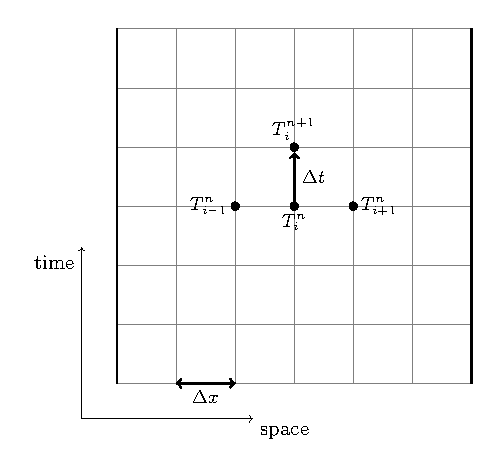
\includegraphics[width=0.5\textwidth]{finitediff}
	\caption{One-dimensional finite-difference schematic. The algorithm is constrained to forward-in-time movement, but varies in both spatial directions. The dark vertical lines at the edge of the schematic are boundary nodes.}
	\label{fig:1DFD}
\end{figure}
Inserting these numerical solutions into Equation \ref{eq:heatdiffusion}, 
the one-dimensional heat diffusion equation can be expressed via a 
finite-difference scheme
\index{Two-Temperature Model!Explicit finite-difference scheme} as
\begin{equation}
\frac{T_{i}^{n+1} - T_{i}^n}{\Delta t} - \alpha \left(\frac{T_{i+1}^{n} - 2T_{i}^n + T_{i-1}^{n}}{\Delta x^2}\right) = \frac{\dot{q}}{C}.
\end{equation}
Rearranging for $T_{i}^{n+1} $ gives
\begin{equation}
T_{i}^{n+1}  = T_{i}^n + \Delta t \bigg[  \alpha \left(\frac{T_{i+1}^{n} - 2T_{i}^n + T_{i-1}^n}{\Delta x^2}\right) + \frac{\dot{q}}{C}  \bigg],
\end{equation}
which is also known as the one-dimensional explicit finite-difference 
solution to Fourier's law of heat conduction. This scheme is illustrated 
in Figure~\ref{fig:1DFD}: it is explicit as the temperature at time $n+1$ 
{\em explicitly} depends on the temperature at time $n$. The 
forward-in-time, space-centred nature of the algorithm is evident in 
Figure~\ref{fig:1DFD}. The timestep and lattice spacing, $\Delta t$ 
and $\Delta x$ respectively, must be chosen carefully to ensure the 
stability of this algorithm, and this is provided by defining the Fourier 
mesh number, $F$, as
\begin{equation}
F = \alpha \frac{\Delta t}{\Delta x^2}
\end{equation}
This can be thought of as the ratio of timestep to the time it takes to 
equilibrate a region of length $\Delta x$. In this one-dimensional 
case, the value of $F$ must satisfy $0 < F < \frac{1}{2}$, or else 
the algorithm becomes unstable and oscillates wildly.

In three-dimensions, if $\Delta x = \Delta y = \Delta z$, the 
finite-difference solution becomes
\begin{align}
T_{i,j,k}^{n+1}  &=& T_{i,j,k}^n + \Delta t \bigg[  \alpha \left(\frac{T_{i+1,j,k}^n + T_{i-1,j,k}^{n} + T_{i,j+1,k}^n + T_{i,j-1,k}^{n} + T_{i,j,k+1}^n + T_{i-1,j,k-1}^{n} - 6T_{i,j,k}^n}{\Delta x^2}\right) + \frac{\dot{q}}{C}  \bigg], \\
T_{i,j,k}^{n+1}  &=& T_{i,j,k}^n + F [T_{i+1,j,k}^n + T_{i-1,j,k}^{n} + T_{i,j+1,k}^n + T_{i,j-1,k}^{n} + T_{i,j,k+1}^n + T_{i-1,j,k-1}^{n} - 6T_{i,j,k}^n] +  \Delta t  \frac{\dot{q}}{C} \label{eq:finite_solver_1},
\end{align}
with a new stability criteria of $0 < F < \frac{1}{6}$. Thus, the size 
of the timestep must satisfy $\Delta t < \frac{\Delta x^2}{6 \alpha}$. 
Equation \ref{eq:finite_solver_1} applies under the assumption that 
the thermal diffusivity $\alpha$ is a constant value, i.e. 
$\nabla . [\alpha \nabla T ] = \alpha \nabla^2 T$, but the more general 
(and hence more complicated) case, where $\alpha$ can vary 
spatially, takes the form
\begin{multline}
T_{i,j,k}^{n+1}  =  \frac{\Delta t}{\Delta x^2}  \frac{\kappa \big[ \frac{1}{2} (T^n_{i+1,j,k} + T^n_{i,j,k})  \big]}{C(T^n_{i,j,k})} (T^n_{i+1,j,k} - T^n_{i,j,k}) + \\ 
\frac{\Delta t}{\Delta x^2}  \frac{\kappa \big[ \frac{1}{2} (T^n_{i-1,j,k} + T^n_{i,j,k})  \big]}{C(T^n_{i,j,k})} (T^n_{i-1,j,k} - T^n_{i,j,k})  + \dots + \Delta t \frac{\dot{q^n_{i,j,k}}}{C^n_{i,j,k}}.
\end{multline}
Here the electronic thermal conductivity has an explicit spatial 
dependence. To simplify this relationship, $\kappa$ can be assumed 
to be constant locally, and is taken to be the average value between 
the current and neighbouring cells. An adaptive timestep is also 
utilised, so at each timestep a fraction of the 'worst case scenario' 
for the Fourier mesh number, $F$, is chosen, ensuring the stability 
of the electronic subsystem.

Various boundary condition choices\index{Two-Temperature Model!boundary conditions} 
are available for the edge cells in Figure \ref{fig:1DFD}, which surround the 
simulation in all three dimensions. These are:
\begin{itemize}
	\item {\em Dirichlet Boundary Conditions}: Also known as 
	infinite-flux boundary conditions, the edge cell is fixed at a 
	finite temperature, $T = T_0$, where $T_0$ is the target 
	(system) emperature. Dirichlet BCs are usually chosen for 
	cascade simulations.
	
	\item {\em Neumann Boundary Conditions}: Also known as 
	zero-flux boundary conditions, the temperature of the edge 
	cell is taken to be the value of its corresponding neighbour, 
	thus $\frac{dT}{dt} = 0$ in this region.
	
	\item {\em Robin Boundary Conditions}: Also known as 
	partial or variable flux boundary conditions, the temperature 
	of the edge cell is taken to be a fixed proportion of the 
	neighbouring cell's temperature. Thus 
	$\frac{dT}{dt} = -k (T-T_0)$, where $k$ is the fraction of 
	the neighbouring temperature that is 'targeted'.
\end{itemize}

The electronic energy contained in a CET voxel can be calculated 
by integrating the volumetric heat capacity between a datum temperature 
(e.g. system temperature) and the local electronic temperature, i.e.
\begin{equation}
E_{e}^{j} = \int_{T_{0}}^{T_{e}^{j}} C_{e} dT.
\end{equation}
A quantity of electronic energy can be added to a voxel by setting the 
local electronic temperature to a new value, such that the integral of 
volumetric heat capacity between the original and new temperatures 
gives the required energy. 

The ionic temperatures $T_i$ and $T_i^{\prime}$ can be calculated 
from kinetic energies of atoms in each voxel, i.e. for cell $j$:
\begin{align}
T_{i}^{j}          &= \frac{\sum_{i \in \vec{x}_j} m_i v_i^2}{3 k_B N} \\
T_{i}^{\prime} &= \frac{\sum_{i \in \vec{x}_j, |v_i | > v_{cut}} m_i v_i^2}{3 k_B N^{\prime}}
\end{align}
where $v_{cut}$ is the cut-off velocity beyond which electronic stopping 
is significant, $N$ is the total number of atoms in the voxel and $N^{\prime}$ 
is the number of atoms in the voxel with velocities greater than $v_{cut}$. 
To account for centre-of-mass drift, the atomic velocities $\vek{v}_i$ 
should be corrected by the voxel's velocity, calculated by 
$\vek{v}^j_{com} = \frac{\sum_{i \in \vec{x}_j} m_i \vek{v}_i}{\sum_{i \in \vec{x}_j} m_i}$.
If there are too few (or no) atoms in the voxel, it is considered to be 
inactive as no definable ionic temperatures can be calculated: the 
corresponding electronic temperature and source terms can be 
omitted in Equation \ref{eq:finite_solver_1}. 

\subsection*{MD system}

The principal idea is to modify the MD equations of motion 
according to Langevin 
dynamics\index{Two-Temperature Model!Inhomogenous Langevin NVT}, 
which describes the movement of particles in a viscous medium. 
This viscous medium will represent the electronic subsystem, and the 
modified equation of motion takes the form
\begin{equation} \label{eq:modifiedlang}
{d \vek{v}_{i}(t) \over d t} = {{\vek{f}_{i}(t)+\vek{R}_{i}(t)} \over
m_{i}} - \chi_{i} \; \vek{v}_{i}(t),
\end{equation}
where $m_i$ and $\vec{v}_i$ are the mass and velocity of atom $i$ 
at time $t$, $\vek{f}_{i}$ is the deterministic force on atom $i$ due 
to the interatomic potential, $\vek{R}_{i}(t)$ is a stochastic force with 
random magnitude and orientation and $m_{i} \chi_{i} \vek{v}_{i}(t)$ 
is the frictional force due to the electrons. These last two terms in 
Equation (\ref{eq:modifiedlang}) are the Langevin modifications to 
Newton's second law, which allow energy to be lost and gained by 
the MD system. 

The stochastic force $\vek{R}_{i}(t)$ returns energy from the 
electrons to the ions and is formulated as 
$\vek{R}_{i}(t) = \sqrt{\Gamma} \vec{A}_{i}(t)$, where $\vec{A}_{i}(t)$ 
is a three-dimensional vector with components randomly distributed 
in $[-1,1]$, and $\Gamma$ is the stochastic friction coefficient. 
$\vek{R}_{i}(t)$ must satisfy two important time-averaged conditions:
\begin{eqnarray}
\langle \vek{R}_{i}(t) \rangle &=& 0, \\
\langle \vek{R}_{i}(t) \cdot \vek{F}_{j}(t^{\prime}) \rangle &\propto& \delta_{ij} \delta (t-t^{\prime}) \label{eq:flucdissip}
\end{eqnarray}
The first condition states that over a significant period of time, 
$\vek{R}_{i}(t)$ must not behave as a net source or sink. Equation 
(\ref{eq:flucdissip}) is known as the fluctuation-dissipation theorem, 
which describes how the drag felt by a particle as it moves through 
a viscous medium can give rise to Brownian motion. In the standard 
homogeneous Langevin thermostat, every atom in the MD simulation 
is thermostatted to a target temperature. The inhomogeneous case 
allows for each atom to be thermostatted to the electronic temperature 
of the corresponding continuum electronic cell. This leads to the 
stochastic friction term\index{Two-Temperature Model!electron-phonon coupling}
\begin{equation}
\Gamma = \frac{6 m_{i} \chi_{ep}^j k_B T_e^j}{\Delta t},
\end{equation}
where $\chi_{ep}^j$ is the electron-phonon friction of the $j^{th}$ 
electronic finite-element cell, $T_e^j$ is the electronic temperature 
of the corresponding cell, $k_B$ is the Boltzmann constant, and 
$\Delta t$ is the timestep. The electron-phonon friction term is thus 
calculated at each point in the finite electronic temperature grid:
\begin{equation} \label{eq:chiep}
\chi_{ep} = \frac{G_{ep} \Delta V}{3 k_B N},
\end{equation}
where $\Delta V$ is the volume of the cell ($\Delta x \Delta y \Delta z$), 
$G_{ep}$ is the electron-phonon coupling constant of the material, and 
$N$ is the number of atoms in the cell. 

The friction term in Equation (\ref{eq:modifiedlang}) is made up of two 
forms of energy loss: the previous discussed electron-phonon friction, 
and electronic stopping, which is inelastic electron scattering of ballistic 
atoms. The total electron friction coefficient $\chi_i$ is given by
\begin{equation}
\chi_{i} = \left\{ \begin{array} {l@{\quad:\quad}l}
\chi_{ep} + \chi_{es} & | v_i | > v_{cut} \\
\chi_{ep} & | v_i | \le v_{cut}
\end{array} \right. ,
\end{equation}
where $\chi_{es}$ is the electronic stopping friction, $\vek{v}_{i}$ is 
the velocity of atom $i$, and $v_{cut}$ is the cut-off velocity for which 
electronic stopping becomes significant. The electronic stopping 
friction term can be calculated in a similar fashion to the electron-phonon 
term:\index{Two-Temperature Model!electronic stopping}
\begin{equation} \label{eq:chies}
\chi_{es} = \frac{G_{s} \Delta V}{3 k_B N^{\prime}}
\end{equation}
where $N^{\prime}$ is the number of atoms in the cell with velocities 
greater than $v_{cut}$.

From Equations (\ref{eq:modifiedlang}), (\ref{eq:chiep}) and (\ref{eq:chies}), 
the differences between the contributions from electron-phonon coupling 
and electronic stopping are evident. Electron-phonon coupling allows energy 
to flow to and from the lattice (depending on the temperature gradient between 
ions and electrons), whereas electronic stopping acts solely as an energy 
loss mechanism for the lattice.
\begin{figure*}[ht] 
	\centering
	{
		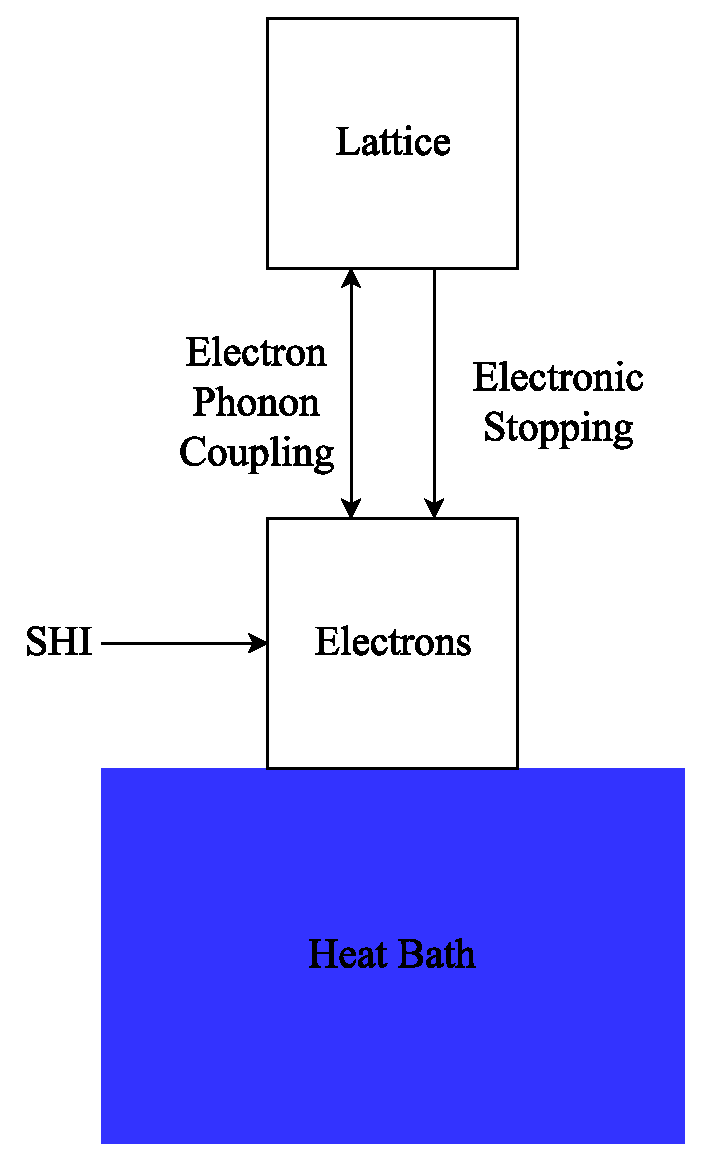
\includegraphics[width=0.3\textwidth]{ttmheatbath}
	}
	\caption{Schematic of thermodynamic coupling and processes in 2T-MD model}
	\label{fig:heatbath}
\end{figure*}
Figure \ref{fig:heatbath} illustrates these processes for swift heavy ion 
simulations, and highlights how the MD cell is now indirectly thermostatted 
to a heat bath. The lattice will reach local equilibrium with the electrons, 
which are thermostatted to the heat bath, thus eventually driving both 
subsystems to the chosen ambient temperature. Energy can only be 
removed from the system via the electrons; this is justified due to how 
slow lattice heat diffusion is in comparison to electronic heat diffusion.

It is possible to use the inhomogeneous Langevin thermostat (Equation 
(\ref{eq:modifiedlang})) on its own\index{ensemble!Inhomogeneous Langevin NVT} 
without coupling it to the electronic temperature grid, but still enhancing 
the total Langevin friction term for atoms with velocities greater than a 
cut-off value\cite{zarkadoula-13a}. In this case, the stochastic friction 
coefficient $\Gamma$ is modified to use the system temperature $T_0$ 
instead of a local electronic temperature and to take advantage of the 
enhanced friction coefficient when electronic stopping applies, i.e.
\begin{equation}
\Gamma = \frac{6 m_{i} \chi_{i} k_B T_0}{\Delta t}.
\end{equation}

\section{Simulation setup}

There are three distinct types of irradiation that can be simulated using 
the TTM (2T-MD) implementation in \D: swift heavy ions, laser excitation, 
and high-energy cascades. These are conducted by splitting the MD cell 
into discrete coarse-grained lattice ionic temperature (CIT) voxels, and 
discretising the electronic system into coarse-grained electronic 
temperature (CET) voxels. Energy can thus be exchanged between the 
voxels and subsequently passed to or from the atoms within each respective 
CIT. The volume of each CIT voxel must contain a sufficient number of atoms 
so that thermal fluctuations of ions are negligible and an ionic temperature 
can be defined: a good general choice is a cube of length 10 \AA in each 
direction. There is more flexibility in choosing the number of CET voxels, 
as long as an integer number of these overlap with the CIT grid: to simplify 
the connections between the CET and CIT grids, equal-sized voxels for both 
systems will be assumed from here on.

\subsection*{Cascades}\index{Two-Temperature Model!cascades}

\begin{figure*}[h] 
	\centering
	{
		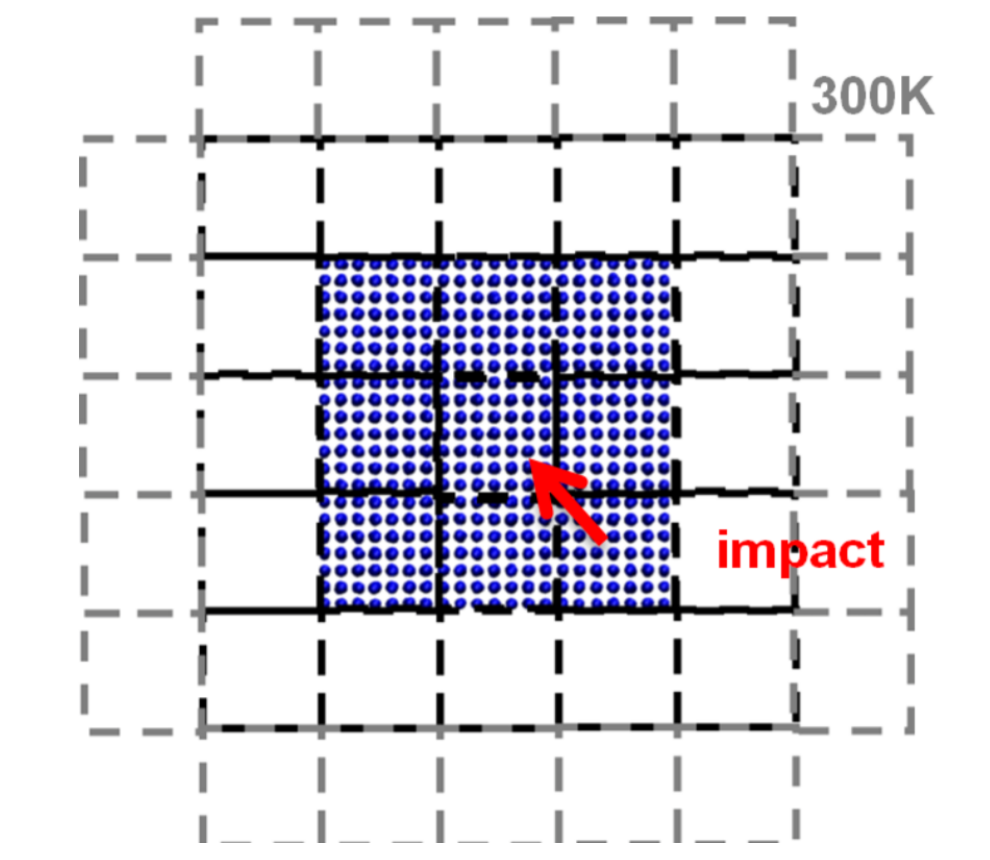
\includegraphics[width=0.3\textwidth]{cascades}
	}
	\caption{Schematic of cascade simulation setup. The electronic temperature cells extend over the ionic (MD) simulation cell to simulate electronic energy dissipation. The boundary conditions of the $T_e$ part are set to converge towards 300K to represent conduction into the bulk.}
	\label{fig:cascades}
\end{figure*}
High-energy cascades require no initial energy deposition into the 
electronic system (i.e. $\frac{dE}{dx} = 0$): instead, an ion is 
initialised with a very high velocity. The electronic temperature 
(CET) voxels extend further than the ionic temperature (CIT) 
voxels in all directions, with open (Dirichlet) or semi-open 
(Robin) boundary conditions in all dimensions to represent thermal 
electronic conduction into the bulk. (Figure~\ref{fig:cascades} gives 
a schematic of this simulation setup.) Stochastic boundary 
conditions can be applied in the ionic system to dampen the shock 
wave generated by the displacement spike.

\subsection*{Swift heavy ions}\index{Two-Temperature Model!swift heavy ions}

\begin{figure*}[h] 
	\centering
	{
		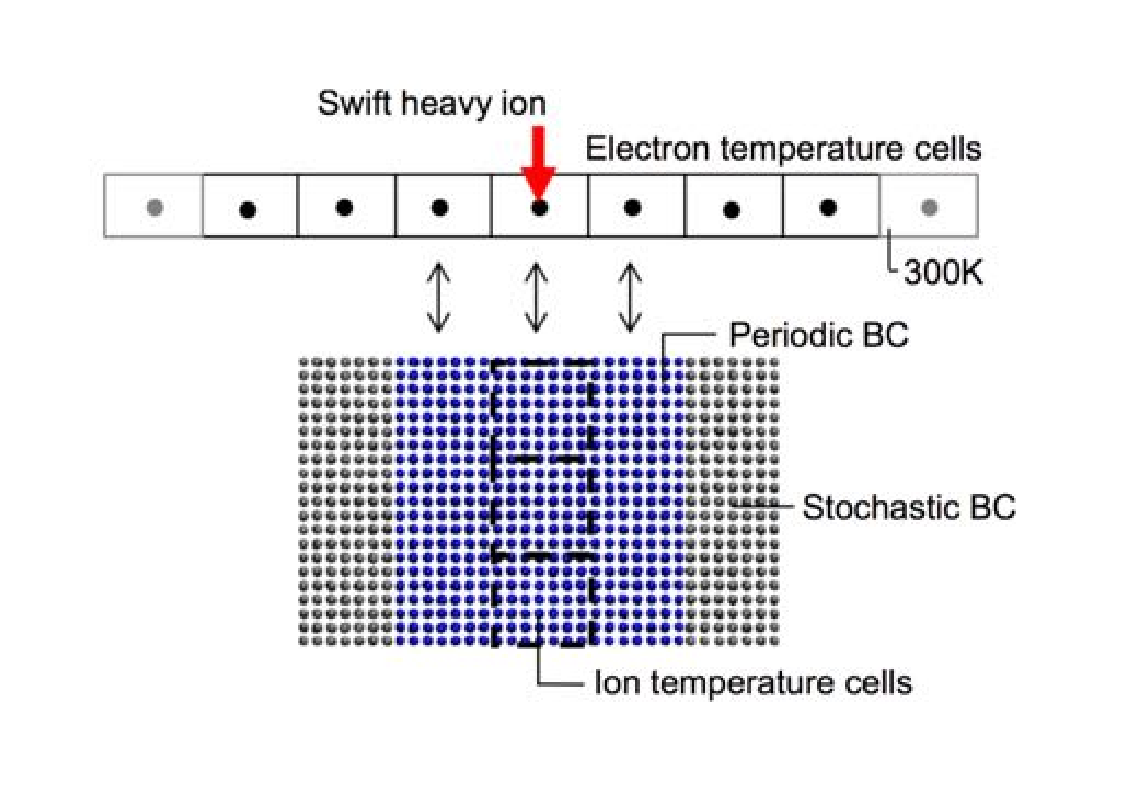
\includegraphics[width=0.5\textwidth]{swiftheavyion}
	}
	\caption{Simulation setup for swift heavy ion impact.}
	\label{fig:SHI}
\end{figure*}
Swift heavy ion systems can be modelled using an initial Gaussian 
spatial energy deposition into the electronic system (i.e. 
$\frac{dE}{dx} > 0$) with either Gaussian or exponentially decaying 
temporal distribution in electronic temperature. The size of the 
electronic temperature (CET) grid in the z-direction is set equal to 
the size of the ionic temperature (CIT) grid in the same dimension, 
while the CET voxels are extended over the corresponding CIT 
voxels in the x- and y-directions. Boundary conditions can be set 
with no energy flux in the z-direction and open or semi-open 
boundary conditions in x- and y-directions. (Figure~\ref{fig:SHI} 
gives a schematic of this simulation setup.) Stochastic boundary 
conditions can be applied to the lattice system in lateral directions 
only to represent non-negligible phononic thermal conductivity 
in semiconductors into the builk. Similarly, while electronic thermal 
conduction in the lateral directions is allowed, conduction parallel to 
impact is not. This reflects the fact that the simulation represents a 
small cross-section of the evolution of a micron-sized track.

\subsection*{Laser excitation}\index{Two-Temperature Model!laser excitation}

\begin{figure*}[h] 
	\centering
	{
		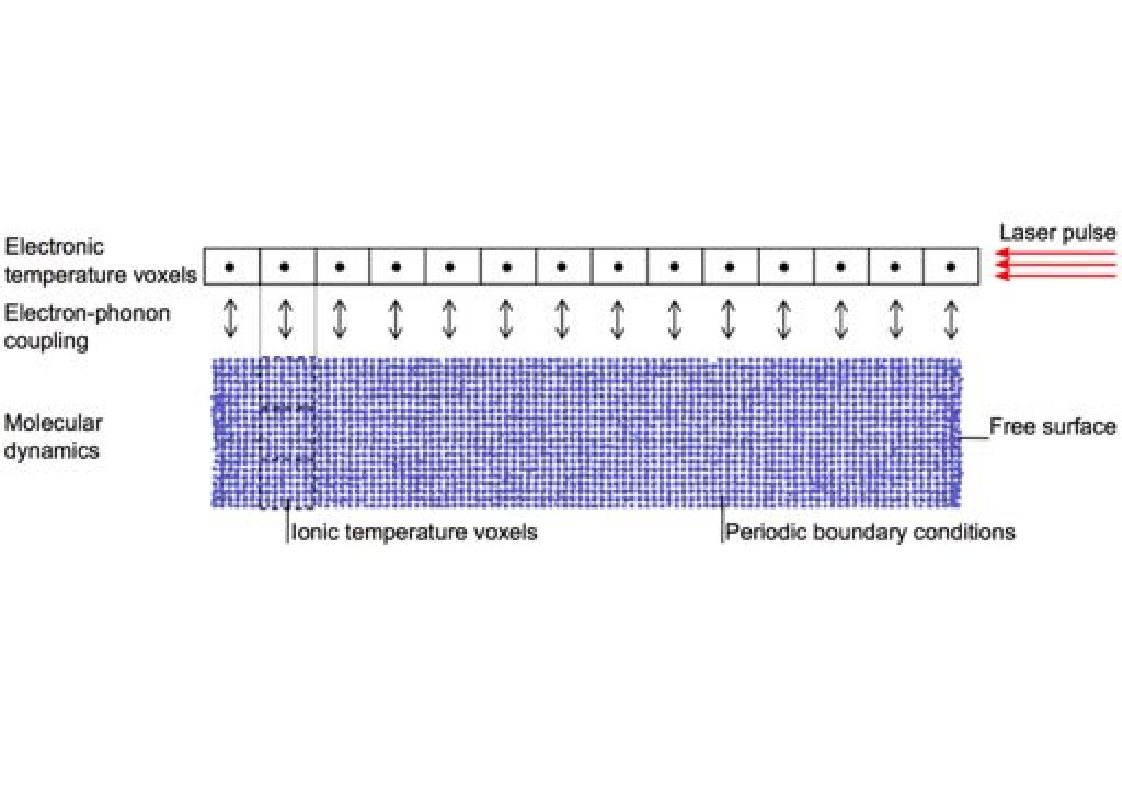
\includegraphics[width=0.7\textwidth]{laser}
	}
	\caption{Simulation setup for laser irradiation.}
	\label{fig:laser}
\end{figure*}
Laser excitation systems can be modelled with an initial homogeneous
spatial energy deposition into the electronic system (either in all three directions
or in x- and y-directions with exponential decay in the z-direction) with either Gaussian 
or exponentially decaying temporal distribution in electronic temperature. 
(The energy deposition can be specified for the fully homogeneous case 
either by setting $\frac{dE}{dx} > 0$ or by giving values for the absorbed fluence 
and penetration depth from the laser.) The size of the electronic temperature (CET) 
grid is set to the same size as the ionic temperature (CIT) grid, with zero-flux 
(Neumann) boundary conditions in all directions. This setup (shown in Figure~\ref{fig:laser}) 
represents a homogeneous laser excitation with the simulated part as a 
small section of a larger photoexcited sample.

\section{Implementation}

The two-temperature (TTM, 2T-MD) model has been implemented in \D
to take advantage of the domain decomposition scheme used by the code,
by dividing up the coarse-grained ionic (CIT) and electronic (CET) 
temperature voxels as evenly as possible among the processors based on 
location. This avoids the need for each processor to hold copies of the 
entire CIT and CET grids and provides good to excellent parallel scalability 
for larger scale problems.

Coarse-grained ionic temperature (CIT) voxels are divided among processors 
with overlapping voxels between two or more processors assigned to the 
first processor in each direction. A boundary halo of voxels is also included 
to allow communication of contributions to voxel momenta, kinetic energies and 
atom counters between processors for calculations of ionic temperatures. Since 
ionic temperatures are only needed for finite-difference calculations of 
Equation (\ref{eq:electronic_system}), some of these communications only 
need to be applied in one direction for each dimension. 

The coarse-grained electronic temperature (CET) grid is considered as 
integer multiples of the ionic temperature grid, with equal numbers in both 
directions of each dimension. While this may provide more CET voxels than 
requested by the user, the application of boundary conditions in the correct
places means that the finite-difference calculations can be carried out in 
superfluous voxels without affecting the result. The centre of the CET grid is 
located at the same place as the CIT grid, matching the two up precisely: the 
electron-phonon, electronic stopping and energy deposition source terms are 
only applied in these CET voxels. Communications of electronic temperature 
can be carried out both within each `copy' of the ionic temperature grid and 
between them: these need to be applied for each iteration (timestep) of the 
finite-difference solver.

Communications to and from boundary halos for both CIT and CET grids 
make use of MPI derived data types, which allow for single MPI send and 
receive calls for grid values without needing to pack and unpack data. This 
is the same communication technique used in DL\_MESO for its lattice 
Boltzmann equation code\cite{seaton-13a} and has been shown to give 
near-perfect parallel scaling to thousands of processors.

\subsection*{Functionality and directives}

All directives in the CONTROL file beginning with {\bf ttm} will switch on 
the two-temperature model (TTM, 2T-MD) as described above. If no other 
information is provided, \D will use default values for certain required 
properties, but some information {\em must} be provided: if this information 
is unavailable, \D will terminate. The list of TTM directives is given as part of 
Section \ref{control_options}: more details about these directives are given 
below.

The inhomogeneous Langevin thermostat can be activated using the 
directive {\bf ensemble~nvt~ttm} or {\bf ensemble~nvt~inhomo} in the 
CONTROL file, specifying the electron-phonon friction term ($\chi_{ep}$, 
in ps$^{-1}$), electronic stopping friction term ($\chi_{es}$, in ps$^{-1}$) 
and the cutoff atomic velocity for electronic stopping ($v_{cut}$, in 
\AA~ps$^{-1}$). This thermostat is required for TTM (2T-MD) calculations 
but can also be used independently: this CONTROL file directive therefore 
does not automatically switch on the two-temperature model, but the 
thermostat will be selected automatically if TTM is otherwise switched on. 
Default values for $\chi_{ep}$, $\chi_{es}$ and $v_{cut}$ will be used in this 
case if they have not been specified, although if a standard NVT Langevin 
ensemble has been selected, its thermostat friction term $\chi$ will be used 
for $\chi_{ep}$. 

By default, the inhomogeneous Langevin thermostat will be applied only to 
particle thermal velocities, i.e. velocities that have been corrected to 
remove the centre-of-mass flow calculated from its coarse-grained ionic 
temperature (CIT) voxel. This can be overridden either by the directive 
{\bf ttm thvelz} to only correct the z-direction velocity component and use 
total velocity components in the x- and y-directions, or by the directive 
{\bf ttm nothvel} to omit all velocity corrections and use total particle 
velocities. A warning message will also be printed if the {\bf no vom} option
is not used, as removal of total centre-of-mass motion may affect the 
dynamics of systems with electronic stopping effects.

The number of coarse-grained electronic temperature (CET) voxels is 
specified in the CONTROL file with the directive {\bf ttm ncet}: by default, 
a grid of $50 \times 50 \times 50$ will be used if this information is not 
supplied by the user. The number of coarse-grained ionic temperature (CIT) 
voxels in the z-direction is specified in CONTROL using the directive 
{\bf ttm ncit}: the default number is 10, and the number of voxels in x- 
and y-directions will be determined automatically based on system size. 
The number of CET voxels must be at least the same as CIT or larger: 
too few CET voxels will cause \D to terminate.

The volumetric heat capacity $C_e$\index{Two-Temperature Model!heat capacity} 
can be obtained for TTM calculations in four different forms with their 
corresponding CONTROL file directives: 
\begin{itemize}
\item A temperature-independent constant value, $C_e = C_0 \rho$ ({\bf ttm ceconst});
\item A linear function of temperature up to a maximum at the Fermi temperature $T_{f}$, $C_e (T) = C_0 \rho \max \left(T/T_{f}, 1\right)$ ({\bf ttm celin});
\item A hyperbolic tangent function of temperature, $C_e (T) = A \rho \tanh \left(10^{-4} B T\right)$ ({\bf ttm cetanh});
\item A tabulated function of temperature supplied in a Ce.dat file  ({\bf ttm cetab}).
\end{itemize}
Note that the values given for the first three options are specific heat 
capacities ($C_0$ and $A$ given in $k_B$ per atom), which are 
converted to volumetric heat capacities by multiplying by the atomic 
density $\rho = \frac{N}{\Delta V}$. The atomic density is assumed to 
be constant throughout the system, and this value can be set in one of three
ways: (1) the user can specifiy a value using the {\bf ttm atomdens} directive 
in the CONTROL file, (2) the value can be calculated 
dynamically from active CITs when using the {\bf ttm dyndens} directive, or 
(3) an unchanging value can be calculated from the provided configuration
at the start (assuming all ionic temperature cells are active). Tabulated 
volumetric heat capacities are given in the Ce.dat file as 
J~m$^{-3}$~K$^{-1}$, which are converted to $k_B$~\AA$^{-3}$. 
If no heat capacity information is supplied, \D will 
assume a constant volumetric heat capacity of 1 $k_B$ per atom by 
default. In all cases, the electronic energy of a given voxel can be 
determined from the product of cell volume and the integral of the 
volumetric heat capacity between the system temperature $T_0$ 
and its current electronic temperature $T_e$.

If the system is metallic (specified by the CONTROL directive {\bf ttm metal}), 
a thermal conductivity\index{Two-Temperature Model!thermal conductivity} 
needs to be supplied: no default value is provided by \D. 
Four options are available with their corresponding CONTROL file directives:
\begin{itemize}
\item An infinitely large value, $K_e = \infty$ ({\bf ttm keinf});
\item A temperature-independent constant value, $K_e = K_0$ ({\bf ttm keconst});
\item A Drude-model (linear) function of temperature, $K_e (T) = K_0 \frac{T}{T_0}$ ({\bf ttm kedrude});
\item A tabulated function of temperature supplied in a Ke.dat file ({\bf ttm ketab}).
\end{itemize}
All values (constants or tabulated) are supplied in W~m$^{-1}$~K$^{-1}$. 
In the case of infinitely large conductivity, all heat diffusion in the electronic 
subsystem is instantaneous and all active CET voxels without source terms 
will be at the same mean electronic temperature. The Drude model uses the 
electronic temperature for a given voxel, while the tabulated function will use 
either the ionic temperature for overlapping cells or the system temperature 
for CET voxels beyond the CIT system. 

If the system is non-metallic (specified by {\bf ttm nonmetal} in CONTROL), 
a thermal diffusivity\index{Two-Temperature Model!thermal diffusivity} 
needs to be supplied: no default value is provided by \D. 
Three options are available with their corresponding CONTROL file directives:
\begin{itemize}
\item A temperature-independent constant value, $D_e = D_0$ ({\bf ttm~deconst} or {\bf ttm~diff});
\item A reciprocal function of temperature up to the Fermi temperature $T_{f}$, $D_e (T) = D_0 \frac{T_0}{\min \left(T, T_{f}\right)}$ ({\bf ttm~derecip});
\item A tabulated function of temperature supplied in a De.dat file ({\bf ttm~detab}).
\end{itemize}
All values (constant and tabulated) are supplied in m$^2$~s$^{-1}$ and 
subsequently converted to \AA$^2$~ps$^{-1}$.

The electron-phonon coupling\index{Two-Temperature Model!electron-phonon coupling} 
friction term $\chi_{ep}$ can either be held at 
the constant value given in {\bf ensemble nvt ttm}, or it can be dynamically 
varied according to electronic temperature. The CONTROL file directive 
{\bf ttm varg} can be used to specify that the electron-phonon coupling 
constant $G_{ep}$ is supplied in tabulated form from a g.dat file, with 
values of $G_{ep}$ given in W~m$^{-3}$~K$^{-1}$ and converted to 
$\chi_{ep}$ values (using Equation (\ref{eq:chiep}) with the mean value for 
the number of atoms per voxel, $N = \rho \Delta V$) in ps$^{-1}$. Two 
variants of dynamic coupling are available: homogeneous coupling 
uses the mean electronic temperature to calculate a system-wide value 
of $chi_{ep}$, while heterogeneous coupling uses local values of 
electronic temperature (based on values in CET voxels) to calculate 
$chi_{ep}$ for each atom.

Boundary conditions\index{Two-Temperature Model!boundary conditions} 
to the electronic temperature system are applied 
using the {\bf ttm bcs} directive in the CONTROL file. Along with the 
Dirichlet, Neumann and Robin boundary conditions described earlier in 
this chapter, periodic boundary conditions can also be applied. 
Combinations of Dirichlet or Robin boundary conditions in x- and 
y-directions with Neumann boundary conditions in the z-direction are 
also available. These boundary conditions have no direct connection to  
any boundary conditions used for the MD system: conditions for the 
latter should be chosen carefully by the user to give the desired effects.

An energy deposition\index{Two-Temperature Model!energy deposition} 
($A(r,t)$) can be applied using one of two CONTROL file directives:
\begin{itemize}
\item {\bf ttm dedx}: specifies the electron stopping power of a projectile entering the electronic system ($\frac{dE}{dx}$ in eV/nm);
\item {\bf ttm laser}: specifies the absorbed fluence ($F$ in mJ~cm$^{-2}$) and penetration depth ($l_p$ in nm) of a laser.
\end{itemize}
The energy deposition can be split into spatial and temporal parts, i.e.
$A(r,t) = f(r,z) g(t) \Delta V$. Depositions can be applied spatially in one of three ways:
\begin{itemize}
\item {\bf ttm sflat}: specifies a homogeneous distribution in x-, y- and z-directions \begin{equation*}f(r) = \frac{dE}{dV} = \frac{dE}{dx} \frac{1}{L_{x} L_{y}}\end{equation*} where $L_{x}$ and $L_{y}$ are the MD system dimensions in x- and y-directions;
\item {\bf ttm sgauss}: specifies a Gaussian distribution in x- and y-directions from the centre of the system, i.e.\begin{equation*}f(r) = \frac{dE}{dx} \frac{1}{2 \pi \sigma^2} e^{-\frac{r^2}{2\sigma^2}}\end{equation*} with standard deviation $\sigma$, extending up to a cut-off distance (given in multiples of $\sigma$);
\item {\bf ttm laser} $F$ $l_p$ {\bf zdep}: specifies a homogeneous distribution in x- and y-directions with exponential decay in the z-direction \begin{equation*}f(r,z) = \frac{F}{l_p} \exp\left(-\frac{z}{l_p}\right) \end{equation*} using the penetration depth $l_p$ as the exponential scaling factor.
\end{itemize}
In the first two cases, spatial depositions are homogeneous in the z-direction. 
Unless the {\bf zdep} option is invoked, laser depositions are homogeneous 
in all three directions (similar to the {\bf ttm sflat} case), with the ratio of 
absorbed fluence to penetration depth equal to $\frac{dE}{dV}$.
The deposition can be applied temporally in one of three ways:
\begin{itemize}
\item {\bf ttm delta}: specifies a Dirac delta function in time \begin{equation*} g(t) = \delta (t - t_0) \end{equation*} which is approximated as an energy injection during a single diffusion timestep;
\item {\bf ttm gauss}: specifies a Gaussian function in time \begin{equation*} g(t) = \frac{1}{\sigma\sqrt{2\pi}}e^{-\left(\frac{t-t_0}{\sigma}\right)^2} \end{equation*} over a period of a multiple of standard deviations $\sigma$;
\item {\bf ttm nexp}: specifies a decaying exponential function in time \begin{equation*} g(t) = e^{-\frac{t-t_0}{\tau}} \end{equation*} over a period of a multiple of $\tau$.
\end{itemize}
The exponential function is scaled to ensure the correct total energy 
(within a tolerance of $\pm 1$\%) is deposited to the electronic system. 
Energy depositions are achieved by determining the required increases 
in electronic temperature to add the required energy to the CET voxel.

To calculate ionic temperatures in CIT voxels, a minimum number of 
atoms is required: this can be specified by the CONTROL file directive 
{\bf ttm amin}, although a default value of 1 is used if this is not supplied 
by the user. Any CIT voxel that includes this number of atoms will be 
considered as active and an ionic temperature can be calculated from 
the mean kinetic energy of atoms in the voxel (after centre-of-mass 
motion is removed). If the voxel does not contain enough atoms, it is 
considered inactive: no electron-phonon coupling is applied to the 
corresponding electronic temperature cell, although thermal diffusion is 
still applied as normal. All voxels within the CIT grid are checked 
at each MD timestep and can be reactivated once the minimum number 
of atoms can be found. If the {\bf ttm dyndens} option is also specified,
the average cell density (number of atoms per cell) will be recalculated 
by only considering active CIT voxels.

If the {\bf ttm redist} option is in use, any recently deactivated voxels 
have their electronic energy transferred to neighbouring active voxels 
by increasing their electronic temperatures: these are used for localised 
Dirichlet (constant temperature) boundary conditions during thermal 
diffusion in the single MD timestep. The corresponding electronic 
temperature cell is also deactivated: its electronic temperature is set to 
the system temperature and the voxel is excluded from thermal diffusion 
calculations by setting the electronic temperature gradient between itself 
and any neighbours to zero. This option requires at least one electronic 
temperature cell beyond the ionic system in each direction to ensure 
electronic energy from deactivated cells is not lost: if this condition 
does not hold, the energy transfer option is switched off.

To equilibrate the electronic system prior to any energy deposition, 
the CONTROL file directive {\bf ttm offset} can be used to allow the 
electronic and ionic systems to settle: this switches off the 
electron-phonon terms in both electronic heat diffusion calculations 
and the inhomogeneous Langevin thermostat, only applying 
electronic stopping effects. The {\bf ttm oneway} directive restricts 
electron-phonon coupling to coarse-grained ionic temperature (CIT) 
voxels and their atoms when the electronic temperature is higher 
than the ionic temperature: both the electron-phonon coupling term 
in the thermal diffusion equation and the inhomogeneous Langevin 
thermostat are switched off if this condition is not met.

The CONTROL file directives {\bf ttm stats} and {\bf ttm traj} switches 
on outputs of statistical information and limited temperature trajectory 
snapshots of the two-temperature model simulation. Ionic 
temperatures (minimum, maximum, mean and sum) are supplied at 
user-defined intervals in the file PEAK\_I, while electronic temperatures 
and energies are supplied in the PEAK\_E file. Ionic and electronic 
temperature profiles along the y-direction at the centre of the xz plane 
are given in the LATS\_I and LATS\_E respectively at user-defined 
intervals.

\subsection*{Overview of program structure}

The following modules, both modified and added, incorporate the 
two-temperature molecular dynamics model in \D:
\begin{itemize}
	\item  {\sc dl\_poly.f90}: modified to initialise {\sc ttm\_module.f90};
	\item  {\sc read\_control.f90}: modified to include the additional control directives required to activate and parameterise TTM;
	\item  {\sc ttm\_module.f90}: deal with initial array allocation, locations of electronic temperature voxel boundaries etc.;
	\item  {\sc ttm\_track\_module.f90}: deal with initial energy deposition to the electronic temperature grid;
	\item  {\sc ttm\_utils.f90}: contains functions to calculate properties for heat diffusion calculations, boundary conditions etc.;
	\item  {\sc ttm\_table\_scan.f90}: scans for any-temperature dependent electronic parameter data files;
	\item  {\sc ttm\_table\_scan.f90}: reads in tabulated parameters for the electronic system;
	\item  {\sc ttm\_system\_init.f90}: reads in any electronic temperature files (DUMP\_E) to allow simulation restart;
	\item  {\sc w\_md\_lfv.f90} and {\sc w\_md\_vv.f90}: modified to calculate ionic lattice and electronic cell temperatures and call the new inhomogeneous Langevin thermostat ({\sc nvt\_l2\_lfv.f90} and {\sc nvt\_l2\_vv.f90});
	\item  {\sc ttm\_ion\_temperatures.f90}: calculates local ion lattice temperatures from average kinetic energies of atoms in coarse-grained ionic temperature (CIT) cells and electronic stopping terms (determining energy transferred from ions to electrons);
	\item  {\sc ttm\_thermal\_diffusion.f90}: calculates local electronic temperatures by solving the heat diffusion equation using a finite-difference solver, including source and sink terms representing energy exchange with the MD cell;
	\item  {\sc w\_integrate\_lfv.f90} and {\sc w\_integrate\_vv.f90}: modified to call the new inhomogeneous Langevin thermostat ({\sc nvt\_l2\_lfv.f90} and {\sc nvt\_l2\_vv.f90});
	\item  {\sc nvt\_l2\_lfv.f90} and {\sc nvt\_l2\_vv.f90}: new inhomogeneous Langevin thermostat (both leap-frog and velocity Verlet variants);
	\item {\sc langevin\_forces.f90}: modified to allow scaling of Langevin random forces by local electronic temperature instead of system temperature;
    \item  {\sc ttm\_system\_revive.f90}: writes file with electronic temperatures (DUMP\_E) to allow the system with TTM to be restarted. 
\end{itemize}
